% Paths assume the manuscript imports from this repository root.
\begin{figure}[t]
  \centering
  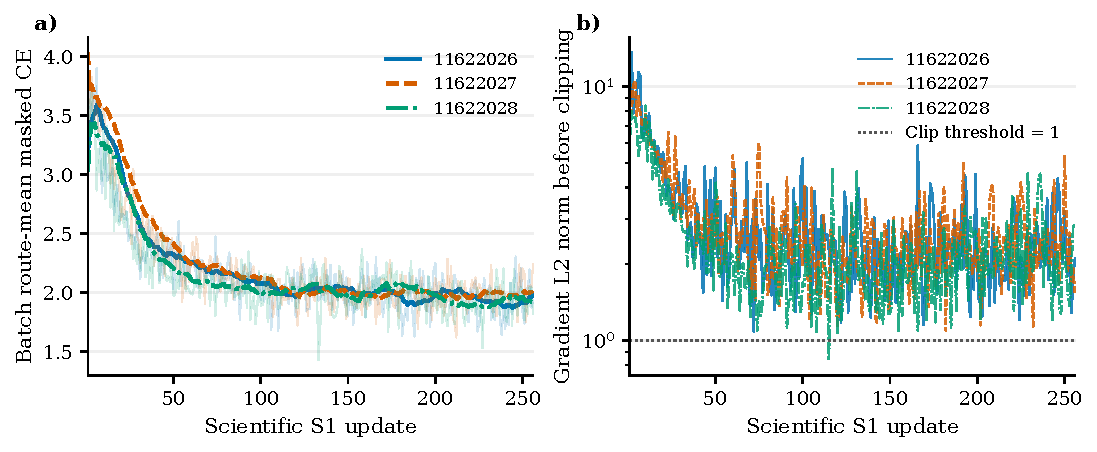
\includegraphics[width=\linewidth]{rc3_s1b_results_20261106/figures/s1b_training_curves.pdf}
  \caption{Actual S1-B training on three fixed optimization seeds. (a) Batch route-mean masked cross entropy: thin traces show all 256 updates; bold traces show the trailing mean of up to 16 updates. (b) Global gradient norms before clipping, with the fixed threshold of one. Changing training batches prevent interpreting individual endpoint batch losses as a paired dataset comparison.}
  \label{fig:s1b-training}
\end{figure}
\begin{figure}[t]
  \centering
  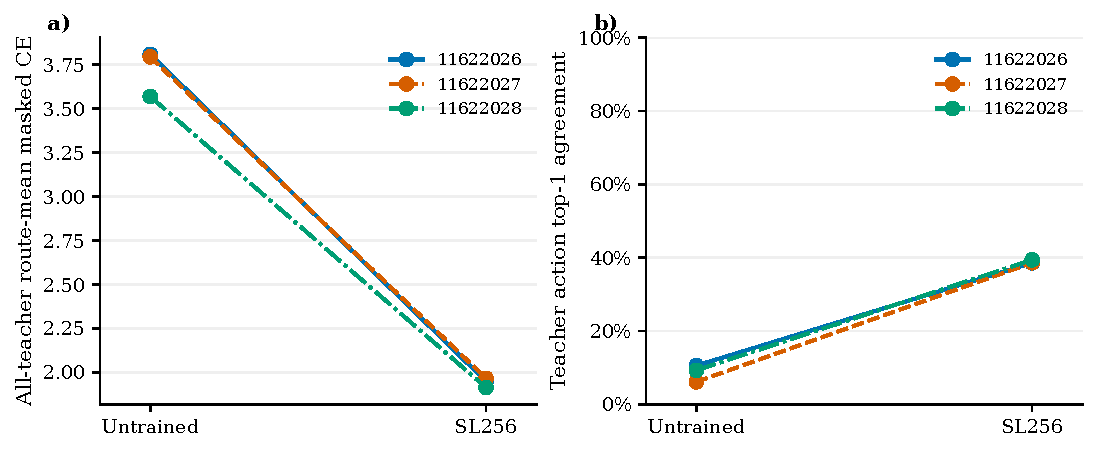
\includegraphics[width=\linewidth]{rc3_s1b_results_20261106/figures/s1b_teacher_agreement.pdf}
  \caption{Paired untrained and fixed SL256 endpoints evaluated on every saved prefix of all 256 S1 training teachers. (a) Route-macro masked cross entropy; (b) state-micro top-1 teacher action agreement. The environment follows teacher actions for both endpoints. These are training-set imitation diagnostics, not independent route-quality, generalization or reinforcement-learning results.}
  \label{fig:s1b-teacher}
\end{figure}
